%==============================================================================
%  A Statistical Thermodynamic Lattice Model for Cu-In Coupled Substitution
%  in Sphalerite
%
%  He Yu (Hezhou University) & Ruqing Chen (GUT Geoservice Inc.)
%
%  Compile:  pdflatex sphalerite_cu_in.tex   (run twice for cross-references)
%  Figures:  ../figures/fig1_annealing.pdf ... fig4_ergodicity.pdf
%==============================================================================
\documentclass[11pt,a4paper]{article}

\usepackage[margin=2.5cm]{geometry}
\usepackage{amsmath,amssymb}
\usepackage{booktabs}
\usepackage{graphicx}
\usepackage{authblk}
\usepackage[round,authoryear]{natbib}
\usepackage{caption}
\usepackage[hidelinks]{hyperref}
\usepackage{url}
\usepackage{setspace}

\graphicspath{{../figures/}{figures/}{./}}

\captionsetup{font=small,labelfont=bf}
\setlength{\parskip}{2pt}

\newcommand{\dQ}{\Delta Q}
\newcommand{\aInCu}{\alpha_{\mathrm{In\text{-}Cu}}}
\newcommand{\RCuIn}{R_{\mathrm{Cu\text{-}In}}}

\title{\bfseries A Statistical Thermodynamic Lattice Model for
Cu--In Coupled Substitution in Sphalerite}

\author[1]{He Yu}
\author[2]{Ruqing Chen\thanks{Corresponding author.}}
\author[3]{Huanzhang Lu}
\affil[1]{Geological Laboratory, Hezhou University, Hezhou, Guangxi 542899, China}
\affil[2]{GUT Geoservice Inc., Montreal, Quebec, Canada}
\affil[3]{D\'epartement des sciences appliqu\'ees et Centre d'\'etudes sur les
ressources min\'erales, Universit\'e du Qu\'ebec \`a Chicoutimi, Quebec, Canada}

\date{}

\begin{document}
\maketitle

\noindent\small
\textit{E-mail addresses:} \texttt{yuhe@hzxy.edu.cn} (H. Yu),
\texttt{ruqing@hotmail.com} (R. Chen), \texttt{hzlu@uqac.uquebec.ca} (H. Lu).
\normalsize

\noindent\small
\textbf{Version 2.0.} This version corrects the equilibration argument of
Section~\ref{sec:ergodicity}. Replica-exchange sampling reaches a state below
anything the annealing protocol of version 1 attained, showing that the
two-trajectory test reported there was not a sufficient test of equilibrium.
Re-measuring both Hamiltonians shows the effect is confined to the full model,
which shifts $\RCuIn$ at 573~K from 24.48 to 25.00, about 2\%; the
electrostatics-only calculation reproduces its published values exactly. That
contrast identifies the hypothetical covalent term, not the charge-compensation
term, as the origin of the sampling difficulty, and
Section~\ref{sec:jdiagnostic} is revised accordingly. No conclusion of version 1
is altered. Full detail in Section~\ref{sec:ergodicity}.
\normalsize


%==============================================================================
\begin{abstract}
\noindent
Indium in sphalerite is almost invariably accompanied by copper in a near-1:1
molar ratio, a relation reproduced across volcanogenic massive sulphide,
Mississippi Valley-type, vein and skarn deposits and universally attributed to
the coupled substitution
$2\,\mathrm{Zn^{2+}} \leftrightarrow \mathrm{Cu^{+}} + \mathrm{In^{3+}}$. The
relation has been documented extensively but never derived: no existing
framework predicts its magnitude, its temperature dependence, or the conditions
under which it should fail. We construct a configurational Hamiltonian for the
sphalerite cation sublattice, $H = E_c + E_s + E_{sub} + E_{def}$, and sample it
by Metropolis Monte Carlo.

An exact topological property of the zinc-blende structure --- that two
nearest-neighbour cations share precisely one bridging anion --- reduces the
charge-compensation term without approximation to a nearest-neighbour pair
interaction whose coefficient is fixed by the dielectric constant of ZnS rather
than fitted, $\lambda = 0.227$--$0.368$~eV. The Cu--In pair binding energy is
$-2\lambda \approx -0.45$ to $-0.73$~eV, and the ground state at Cu:In~$=1$:1 is
shown analytically to be exactly the roquesite ($\mathrm{CuInS_2}$) cation
ordering, recovered without any input describing that structure.

Simulations at 2~at.\% substitution reproduce these predictions. Electrostatics
alone enriches Cu--In nearest-neighbour bonds sixteenfold over the random solid
solution at $300\,^\circ$C and removes 96\% of the local charge imbalance;
heterovalent bonds are enriched 2.7 times more strongly than homovalent ones.
Elastic terms, retained at full strength in a control calculation, produce no
detectable ordering. The ordering crossover lies at a reduced temperature three
to seven times above the entire hydrothermal window, so short-range order is
saturated wherever sphalerite forms and carries no thermometric information.

Three consequences follow: indium tenor should be limited by the availability of
a monovalent charge compensator rather than by indium supply; vacancy
compensation, disfavoured electrostatically by $8\lambda \approx 2.4$~eV, should
be diagnostic of copper-poor systems and detectable as cation deficiency; and
the ideal dilute-mixing entropy assumed in conventional partition-coefficient
models is substantially overestimated. Finite box size prevents resolution of
the solid-solution versus nanoinclusion boundary, which we identify as the
specific target of large-scale simulation.

\vspace{4pt}
\noindent\textit{Keywords:} sphalerite; indium; coupled substitution; charge
compensation; statistical thermodynamics; Monte Carlo; roquesite; critical
metals
\end{abstract}

%==============================================================================
\section{Introduction}

\subsection{An empirical regularity without a derivation}

Among the trace-element relations recorded in sulphide minerals, few are as
reproducible as the coupling between copper and indium in sphalerite. Across
volcanogenic massive sulphide, Mississippi Valley-type, vein and skarn systems,
and over concentration ranges spanning several orders of magnitude,
laser-ablation ICP-MS analyses of sphalerite return Cu and In in a molar ratio
close to unity \citep{cook2009,frenzel2016}. The relation is sufficiently
consistent that
departures from it are themselves treated as diagnostic, and it is universally
interpreted in terms of the coupled substitution
\begin{equation}
2\,\mathrm{Zn^{2+}} \;\longleftrightarrow\; \mathrm{Cu^{+}} + \mathrm{In^{3+}},
\label{eq:coupled}
\end{equation}
with a subordinate vacancy-compensated mechanism,
$3\,\mathrm{Zn^{2+}} \leftrightarrow 2\,\mathrm{In^{3+}} + V_{\mathrm{Zn}}$,
invoked where the ratio departs from unity
\citep{johan1988,belissont2014}.

What has not been established is why. Equation~\eqref{eq:coupled} is a statement
of stoichiometry, not of energetics: it specifies that charge balance must be
maintained somewhere in the crystal, but it says nothing about whether Cu and In
should occupy adjacent sites or opposite ends of the grain, how strongly they
should be associated, how that association should vary with temperature, or
under what conditions the alternative mechanism should take over. These are
precisely the questions on which the geological utility of the observation
depends, and answering them requires a statistical-mechanical treatment of the
cation sublattice rather than a balanced chemical equation.

\subsection{Why the answer matters beyond mineral chemistry}

Indium is classified as a critical raw material in most national assessments,
and its supply is unusual in that it is essentially never mined for its own
sake: there are no indium ores in the conventional sense, and the overwhelming
majority of primary production is recovered as a by-product of zinc refining
\citep{werner2015,usgs2024}. The consequence is
that the global indium endowment is not controlled by a distinct ore-forming
process at all, but by the trace-element chemistry of sphalerite --- that is, by
the site-occupancy problem posed above. Predicting where indium is concentrated
is therefore, quite literally, a problem of predicting the internal
configurational state of a mineral.

This inverts the usual relationship between mineral physics and economic
geology. For most commodities the mineralogy is a consequence of the ore process
and can be treated as a downstream detail; for indium, the mineralogy \emph{is}
the ore process. It follows that a predictive theory of trace-element
incorporation in sphalerite is not a refinement of exploration practice but a
prerequisite for it.

\subsection{The theoretical bottleneck}

Existing approaches fall into three groups, none of which addresses the
configurational question directly.

The first is empirical partitioning. Deposit-type meta-analyses and
temperature-calibrated distribution coefficients summarise observed
concentrations and their controls with considerable success
\citep{frenzel2016}, but they are
descriptive by construction. They cannot predict behaviour outside the
calibrated range, and --- as shown in Section~\ref{sec:exploration} --- the
ideal dilute-mixing entropy on which such treatments implicitly rest is not a
good approximation for a system with the degree of short-range order reported
here.

The second is micro-analytical mapping. High-resolution LA-ICP-MS imaging and
electron microscopy have established that indium is often distributed
heterogeneously within single grains, and have raised the still-unresolved
question of whether it resides in genuine solid solution or in nanoscale
inclusions of a discrete In phase such as roquesite \citep{moura2007}.
This debate has proved difficult to settle empirically because the two states
differ at length scales at the limit of detection. What has been missing is a
theoretical criterion predicting which state should occur, and under what
conditions.

The third is first-principles defect chemistry. Density-functional calculations
of point defects in ZnS and related II--VI semiconductors provide substitution
and formation energies of the kind required
\citep{freysoldt2014,hoang2019}, but they characterise isolated or paired defects in
periodic supercells. They do not, and are not intended to, describe the
statistics of $10^{2}$--$10^{5}$ mutually interacting substituents at finite
temperature. The step from defect energetics to mineral chemistry is a
configurational-statistics problem, and it is that step which is absent from the
literature.

The gap, stated compactly, is this: the mineralogical community possesses
extensive observations of Cu--In coupling and the physics community possesses
the energetics of individual defects, but no framework connects the two. This
paper is an attempt to supply one.

\subsection{Approach and principal findings}

We construct a four-term configurational Hamiltonian on the sphalerite cation
sublattice,
\begin{equation}
H = E_c + E_s + E_{sub} + E_{def},
\label{eq:H}
\end{equation}
in which $E_c$ penalises departures from local electroneutrality within each
anion coordination tetrahedron, $E_s$ represents elastic misfit in the Eshelby
continuum approximation, $E_{sub}$ carries the chemical cost of substitution
referenced to the ore fluid, and $E_{def}$ describes cation vacancies. The
Hamiltonian is sampled by Metropolis Monte Carlo with Kawasaki exchange
dynamics, and validated against a suite of analytic limits that it reproduces to
machine precision.

Two features distinguish the treatment from a phenomenological lattice model.
First, the charge-compensation term is not postulated but derived: an exact
topological property of the zinc-blende structure allows the tetrahedral
electroneutrality functional to be reduced, without approximation, to a
composition constant plus a nearest-neighbour pair interaction, whose
coefficient is then fixed by the measured dielectric constant of ZnS rather than
fitted. Second, the model's ground state is determined analytically, and proves
to be the roquesite cation ordering, obtained without any structural input
describing that phase.

The principal findings are:
\begin{enumerate}\itemsep2pt
\item The Cu--In pair binding energy is $-2\lambda \approx -0.45$ to
      $-0.73$~eV, an order of magnitude larger than $k_BT$ at hydrothermal
      temperatures, and contains no adjustable parameter.
\item Charge compensation alone --- with all chemical interaction terms switched
      off --- enriches Cu--In nearest-neighbour bonds sixteenfold over the
      random solid solution at $300\,^\circ$C and eliminates 96\% of the local
      charge imbalance.
\item Elastic misfit, retained at full strength in a control calculation,
      produces no detectable ordering. Cu--In coupling in sphalerite is
      electrostatic, not elastic; the corollary is that Ag--In coupling, with a
      twentyfold larger size mismatch, should behave qualitatively differently.
\item The ordering crossover lies at a reduced temperature three to seven times
      above the entire hydrothermal ore-forming window, so short-range order is
      saturated wherever sphalerite forms and carries no thermometric
      information.
\item The Cu-compensated substitution is favoured over the vacancy-compensated
      route by $8\lambda \approx 2.4$~eV in electrostatic energy, yielding a
      quantitative and falsifiable criterion for the crossover between the two
      mechanisms.
\end{enumerate}

The calculations are deliberately minimal. They use a $10\times10\times10$-cell
box at a single composition, and we show explicitly that this is sufficient to
establish the ordering physics but insufficient to resolve the solid-solution
versus nanoinclusion boundary, because the solute population is exhausted by a
single condensed domain. Rather than obscure this limitation we quantify it, and
use it to specify the box size, sampling algorithm and parameterisation that
addressing the question properly would require.

\subsection{Epistemic conventions}

Every entry of the parameter table (Table~\ref{tab:params}) carries one of three
designations in its \emph{Basis} column, and each subsection of
Section~\ref{sec:theory} closes with a one-sentence statement of the evidential
basis of its content:
\begin{itemize}\itemsep1pt
\item \textbf{[F] Established fact.} Crystallographic, spectroscopic or elastic
      data from the published literature, or an exact mathematical consequence
      of the zinc-blende topology.
\item \textbf{[I] Inference.} A quantity derived from [F] inputs through a
      standard and independently validated physical framework, with no free
      parameters introduced.
\item \textbf{[H] Hypothesis.} An original assumption of this work, not yet
      constrained by measurement or first-principles calculation. Every [H]
      quantity is either scanned over a range or explicitly flagged as requiring
      \textit{ab initio} determination.
\end{itemize}
This convention is retained deliberately: the central claim of the paper is that
the observed Cu--In association follows from [F] and [I] alone, and the
labelling makes that claim falsifiable rather than rhetorical.

%==============================================================================
\section{Theory}
\label{sec:theory}

\subsection{Nomenclature and configurational variables}

Sphalerite crystallises in space group $F\bar{4}3m$ with a cubic cell parameter
$a_0 = 5.4093$~\AA{} for the pure ZnS end-member. The cation sublattice is
face-centred cubic with coordination numbers $Z_1 = 12$ at
$d_{NN} = a_0/\sqrt{2} = 3.825$~\AA{} and $Z_2 = 6$ at $a_0$ \citep{shannon1976};
the sulphur sublattice is a second fcc array displaced by
$(\tfrac14,\tfrac14,\tfrac14)$, so that every S anion is tetrahedrally
coordinated by four cations and every cation by four anions.

We assign to each cation site $i$ a configurational variable
$\sigma_i \in \{\mathrm{Zn}, \mathrm{Cu}, \mathrm{In}, \square\}$, where
$\square$ denotes a cation vacancy $V_{\mathrm{Zn}}$. The associated formal
charges are $q_\alpha = \{2, 1, 3, 0\}$, and we work throughout with the charge
deviation from the host cation,
\begin{equation}
\delta q_i \equiv q_{\sigma_i} - q_{\mathrm{Zn}} = \{0,\, -1,\, +1,\, -2\},
\end{equation}
so that $\delta q_i = 0$ identically on the undisturbed lattice. A configuration
is the complete assignment $\{\sigma\}$ over the $N$ cation sites; there are $N$
anion tetrahedra, indexed by $a$, and $T(a)$ denotes the set of four cations
coordinating anion $a$.

\textit{Basis: the structural data and connectivity are established facts~[F];
the configurational variables are definitions.}

\subsection{A topological lemma}
\label{sec:lemma}

The reduction developed below rests on a single exact property of the
zinc-blende connectivity, which is not, to our knowledge, exploited in existing
lattice treatments of coupled substitution:

\begin{quote}
\textbf{Lemma.} In the zinc-blende structure, two cations are nearest neighbours
if and only if they share exactly one common anion tetrahedron; second- and
higher-neighbour cations share none. Each cation belongs to exactly four
tetrahedra.
\end{quote}

The lemma follows by direct enumeration of the twelve nearest-neighbour vectors
against the four anion offsets, and is asserted computationally over all
neighbours of every site in the implementation of Section~\ref{sec:vv}. Its
consequence is that any energy functional defined on anion tetrahedra maps
\emph{exactly}, with no truncation, onto a composition term plus a
nearest-neighbour pair interaction on the cation sublattice.

\textit{Basis: an exact consequence of the zinc-blende topology~[F].}

\subsection{Local charge compensation, \texorpdfstring{$E_c$}{Ec}}

\subsubsection{From screened electrostatics to a local functional}

Aliovalent substituents in a semiconducting host interact through a Coulomb
potential screened by the dielectric response of the lattice and by any free
carriers present:
\begin{equation}
E_c^{\mathrm{Coul}} = \frac{1}{2}\,\frac{e^2}{4\pi\epsilon_0\epsilon_r}
\sum_{i \neq j} \frac{\delta q_i\, \delta q_j\, e^{-r_{ij}/\ell_D}}{r_{ij}} .
\end{equation}
For defect charges in ZnS the screening length is of the order of the
nearest-neighbour separation, so the series is dominated by the first
coordination shell. Truncating there and invoking the Lemma, we adopt the local
electroneutrality functional
\begin{equation}
\boxed{\;E_c = \lambda \sum_{a=1}^{N} \left( \dQ_a \right)^2 ,
\qquad \dQ_a = \sum_{i \in T(a)} \delta q_i \;}
\label{eq:Ec}
\end{equation}
which penalises departures from charge neutrality within each anion coordination
tetrahedron. This is the lattice-discrete expression of Pauling's second rule,
and $\dQ_a$ is the excess of the bond-valence sum reaching anion $a$ over its
ideal value of two valence units \citep{pauling1929}.

\subsubsection{Exact reduction to a pair interaction}

Expanding the square and applying the Lemma --- each cation appears in four
tetrahedra, and each nearest-neighbour pair co-occurs in exactly one tetrahedron
where it contributes both orderings --- gives the \emph{exact} identity
\begin{equation}
E_c = \underbrace{4\lambda \sum_i \delta q_i^{\,2}}_{\text{composition only}}
 + \underbrace{2\lambda \sum_{\langle ij \rangle} \delta q_i\, \delta q_j}_{\text{nearest-neighbour pair term}} .
\label{eq:Ecpair}
\end{equation}
Two consequences follow. First, at fixed composition the first term is a
constant, so all configurational physics carried by $E_c$ resides in the pair
term; the charge-compensation problem is therefore isomorphic to a four-state
nearest-neighbour Ising-like model with couplings
$J^{c}_{\alpha\beta} = 2\lambda\, \delta q_\alpha \delta q_\beta$. Second, the
interaction is \emph{strictly} nearest-neighbour: no approximation or cutoff has
been imposed beyond the initial truncation of the screened Coulomb series.

\subsubsection{A parameter-free estimate of \texorpdfstring{$\lambda$}{lambda}}

Matching the pair term of Eq.~\eqref{eq:Ecpair} to the nearest-neighbour term of
the screened Coulomb series yields
\begin{equation}
\lambda = \frac{e^2}{8\pi\epsilon_0\,\epsilon_r\, d_{NN}} .
\label{eq:lambda}
\end{equation}
With $e^2/4\pi\epsilon_0 = 14.400$~eV\,\AA{} and $d_{NN} = 3.825$~\AA{}, the
static and high-frequency dielectric constants of ZnS ($\epsilon_0 = 8.3$,
$\epsilon_\infty = 5.13$; \citealp{berlincourt1963,li1984}) bracket
\begin{equation}
\lambda \in [\,0.227,\; 0.368\,]\ \mathrm{eV}.
\end{equation}
$\lambda$ is therefore \emph{not} a fitted parameter. Residual uncertainty
enters through the choice of screening length --- retaining
$e^{-d_{NN}/\ell_D}$ explicitly would reduce $\lambda$ by a factor of order
$e^{-1}$ for $\ell_D \simeq d_{NN}$ --- and through the neglect of Fe~$3d$
states, which modify the dielectric response of natural, Fe-bearing sphalerite.
For this reason $\lambda$ is scanned over $[0, 0.5]$~eV in
Section~\ref{sec:lambdascan}.

\subsubsection{Analytical predictions}
\label{sec:analytic}

Equation~\eqref{eq:Ecpair} admits exact results for small defect complexes, all
verified numerically in Section~\ref{sec:vv} as regression tests. Writing
energies relative to the defect-free lattice:

\begin{center}
\small
\begin{tabular}{lll}
\toprule
Configuration & $E_c$ & Origin \\
\midrule
Isolated $\mathrm{Cu^{+}}$ or $\mathrm{In^{3+}}$ & $4\lambda$ & $4\lambda\,\delta q^2$ \\
Isolated $V_{\mathrm{Zn}}$ & $16\lambda$ & $\delta q = -2$ \\
Nearest-neighbour Cu--In pair & $6\lambda$ & $8\lambda - 2\lambda$ \\
Ground state of $2\mathrm{Cu} + 2\mathrm{In}$ & $8\lambda$ & four Cu--In bonds \\
Ground state of $V_{\mathrm{Zn}} + 2\mathrm{In}$ & $16\lambda$ & two $\square$--In bonds \\
\bottomrule
\end{tabular}
\end{center}

\noindent
The binding energy of the elementary coupled-substitution unit is therefore
\begin{equation}
\Delta E_c^{\,\mathrm{Cu-In}} = -2\lambda \simeq -0.45 \ \text{to} \ -0.73\ \mathrm{eV},
\label{eq:binding}
\end{equation}
an association energy an order of magnitude larger than $k_B T$ at hydrothermal
temperatures ($k_BT = 0.049$~eV at $300\,^\circ$C). The ground state of the
four-defect complex, $8\lambda$, lies below that of two independent pairs
($12\lambda$) because a configuration in which both Cu are nearest neighbours of
both In neutralises four tetrahedra rather than two; clustering beyond the pair
is thus electrostatically favoured from the outset, without recourse to any
attractive chemical term.

\subsubsection{The ground state of \texorpdfstring{$E_c$}{Ec} is the roquesite ordering}
\label{sec:groundstate}

At $x_{\mathrm{Cu}} = x_{\mathrm{In}}$ the charge-compensation term possesses an
exact zero-energy ground state: $E_c = 0$ whenever every anion tetrahedron
contains two Cu and two In, since then $\dQ_a = -1-1+1+1 = 0$ for all $a$. This
is precisely the adamantine cation-ordering rule of chalcopyrite-structured
$\mathrm{CuInS_2}$ --- the mineral roquesite, which is the observed exsolution
product of In-rich sphalerite \citep{moura2007}. We regard this as the central structural result
of the model: \emph{the lowest-energy state of a purely electrostatic local
neutrality functional on the zinc-blende cation sublattice is the roquesite
structure}, obtained without any input describing that structure.

The ground state is, however, degenerate. Any cation ordering satisfying the
$2\mathrm{Cu} + 2\mathrm{In}$ rule attains $E_c = 0$; we verify numerically that
both the chalcopyrite-type ordering and a $\mathrm{CuAu\text{-}I}$-type layered
ordering along $[001]$ do so exactly. Selection among these polytypes must
therefore be made by $E_s$ and $E_{sub}$, and constitutes a well-posed question
for first-principles calculation.

\subsubsection{Competition between compensation mechanisms}
\label{sec:competition}

Two charge-balancing routes for $\mathrm{In^{3+}}$ are documented in natural
sphalerite: monovalent-cation coupling, Eq.~\eqref{eq:coupled}
\citep{johan1988}, and vacancy compensation \citep{trofimov2020}. Both are contained in the present formalism without additional
parameters, because $\delta q_\square = -2 = 2\,\delta q_{\mathrm{Cu}}$.
Comparing the two routes at fixed In content, the table of
Section~\ref{sec:analytic} gives $E_c^{(\mathrm{Cu})} = 8\lambda$ against
$E_c^{(\square)} = 16\lambda$, an electrostatic preference of
$8\lambda \approx 2.4$~eV for the Cu-compensated route. Since the routes differ
in atom count, the full thermodynamic comparison requires the reservoir terms of
Section~\ref{sec:esub}, and the Cu route dominates whenever
\begin{equation}
2\left( \Delta E^{f}_{\mathrm{Cu}} - \mu_{\mathrm{Cu}} \right) - E^{f}_{V}
\;<\; 8\lambda .
\label{eq:crossover}
\end{equation}
Equation~\eqref{eq:crossover} is a falsifiable prediction: vacancy compensation
should be confined to Cu-poor systems, and the crossover should occur at a Cu
activity that the model specifies quantitatively once $E^f_V$ and
$\Delta E^f_{\mathrm{Cu}}$ are known.

\textit{Basis: Eqs.~\eqref{eq:Ec}--\eqref{eq:Ecpair} and the tabulated complex
energies are exact consequences of the Lemma~[F]; the value of $\lambda$ in
Eq.~\eqref{eq:lambda}, the identification of the $E_c$ ground state with the
roquesite ordering, and the criterion of Eq.~\eqref{eq:crossover} are
parameter-free inferences~[I]; the occurrence of both compensation mechanisms in
natural sphalerite is an established fact~[F].}

\subsection{Elastic strain energy, \texorpdfstring{$E_s$}{Es}}

Substituent cations differ in size from the host, and the resulting elastic
energy is treated in the Eshelby continuum approximation for a spherical
misfitting inclusion in an isotropic matrix \citep{eshelby1957}:
\begin{equation}
E_s^{\mathrm{self}} = \sum_i \frac{24\pi\, \mu_m K_p R^3\, \varepsilon_{\sigma_i}^2}{3K_p + 4\mu_m},
\qquad
\varepsilon_\alpha = \frac{r_\alpha - r_{\mathrm{Zn}}}{r_{\mathrm{Zn}}},
\label{eq:eshelby}
\end{equation}
where $R = (3\Omega_0/4\pi)^{1/3} = 2.11$~\AA{} is the Wigner--Seitz radius of a
cation site ($\Omega_0 = a_0^3/4$), and $K = 77$~GPa, $\mu = 30.7$~GPa are the
bulk and Voigt--Reuss--Hill shear moduli of ZnS \citep{berlincourt1963}.
Strain-mediated coupling between
substituents is represented at leading (elastic-dipole) order by a pair term
decaying as $r^{-3}$,
\begin{equation}
E_s^{\mathrm{pair}} = \Gamma \sum_{i<j} \varepsilon_{\sigma_i}\varepsilon_{\sigma_j}
\left( \frac{a_0}{r_{ij}} \right)^{3},
\label{eq:dipole}
\end{equation}
truncated at the second coordination shell, so that
$\Gamma_2 = \Gamma_1 / 2^{3/2}$. The sign structure of Eq.~\eqref{eq:dipole}
encodes strain compensation: substituents of opposite misfit attract, those of
like misfit repel.

Inserting Shannon effective ionic radii for fourfold coordination
\citep{shannon1976},
$r_{\mathrm{Zn^{2+}}} = r_{\mathrm{Cu^{+}}} = 0.60$~\AA{} and
$r_{\mathrm{In^{3+}}} = 0.62$~\AA{}, gives $\varepsilon_{\mathrm{Cu}} = 0.000$
and $\varepsilon_{\mathrm{In}} = +0.033$, whence
$E_s^{\mathrm{self}}(\mathrm{In}) = 0.033$~eV. Comparison with
Eq.~\eqref{eq:binding} gives
\begin{equation}
\frac{E_s^{\mathrm{self}}(\mathrm{In})}{\left| \Delta E_c^{\mathrm{Cu-In}} \right|} \approx 0.05 ,
\end{equation}
which motivates the first original hypothesis of this work:

\begin{quote}
\textbf{Hypothesis H1.} Cu--In coupled substitution in sphalerite is
\emph{electrostatically} rather than \emph{elastically} driven, with the strain
contribution below 10\% of the charge-compensation energy. The corollary is that
Ag--In coupling, for which $\varepsilon_{\mathrm{Ag^{+}}} = +0.67$ and the
linear-elastic treatment itself becomes marginal, should behave qualitatively
differently and should depart from strict 1:1 stoichiometry.
\end{quote}

H1 is falsifiable by first-principles substitution energies, and we test its
internal consistency in Section~\ref{sec:elastic} by comparing the full model
against a calculation in which the chemical and elastic terms are switched off
entirely.

\textit{Basis: the ionic radii and elastic moduli are measured quantities~[F]
and Eqs.~\eqref{eq:eshelby}--\eqref{eq:dipole} apply a standard continuum
framework to them~[I]; the coupling constant $\Gamma_1$ and Hypothesis H1 itself
are assumptions of this work~[H].}

\subsection{Substitutional energy, \texorpdfstring{$E_{sub}$}{Esub}}
\label{sec:esub}

The chemical cost of exchanging a host cation for a substituent, referenced to
external reservoirs, is written in the standard point-defect form
\begin{equation}
E_{sub} = \sum_\alpha N_\alpha \left( \Delta E^{f}_{\alpha} - \mu_\alpha \right)
 + \sum_{\langle ij \rangle} J_{\sigma_i \sigma_j},
\label{eq:esub}
\end{equation}
where $N_\alpha$ is the number of sites occupied by species $\alpha$ and
$\mu_\alpha$ the corresponding chemical potential imposed by the ore fluid. The
formation energies are defined so as to interface directly with supercell DFT
\citep{freysoldt2014},
\begin{equation}
\Delta E^{f}_{\alpha} = E_{\mathrm{def}} - E_{\mathrm{bulk}}
+ \sum_\beta n_\beta \mu_\beta + q\left( E_F + E_{\mathrm{VBM}} \right) + E_{\mathrm{corr}},
\label{eq:dft}
\end{equation}
with $E_{\mathrm{corr}}$ the finite-size electrostatic correction. In the
canonical ensemble used here the reservoir terms are constants and do not
influence the configurational statistics; Eq.~\eqref{eq:esub} is retained in
full because a grand-canonical treatment, in which they control the equilibrium
In content, is the natural extension of this work.

The matrix $J_{\alpha\beta}$ carries all short-range chemical interaction
\emph{beyond} the electrostatics already contained in $E_c$ --- principally
Cu~$3d$--In~$5s$--S~$3p$ hybridisation, which has no counterpart in a
formal-charge description. In the absence of \textit{ab initio} constraint we
adopt $J_{\mathrm{Cu\text{-}In}} = -0.10$~eV and
$J_{\mathrm{Cu\text{-}Cu}} = J_{\mathrm{In\text{-}In}} = +0.05$~eV, i.e.\ a
modest covalent stabilisation of the heterovalent pair and a modest repulsion
between like substituents. Because these are the only genuinely unconstrained
interaction parameters in the model, all principal results are reported both
with and without them.

\textit{Basis: Eqs.~\eqref{eq:esub}--\eqref{eq:dft} are standard
defect-thermodynamic definitions~[F]; the values of $J_{\alpha\beta}$ are
hypotheses of this work~[H].}

\subsection{Defect term, \texorpdfstring{$E_{def}$}{Edef}}

Cation vacancies are treated on the same footing as substituents,
\begin{equation}
E_{def} = \sum_i \delta_{\sigma_i, \square}
\left( E^{f}_{V} + \sum_{j \in NN(i)} w_{\sigma_j} \right),
\end{equation}
where $E^f_V$ is the isolated vacancy formation energy and $w_{\sigma}$ a
short-range association correction. The dominant vacancy--solute association is
already captured by $E_c$ through $\delta q_\square = -2$, so $w_\sigma$ carries
only the non-electrostatic residue and is set to zero at this stage. Vacancy
relaxation is represented through an effective negative misfit
$\varepsilon_\square = -0.20$ entering Eq.~\eqref{eq:eshelby}.

\textit{Basis: the electrostatic part of vacancy--solute association follows from
$E_c$~[I]; $E^f_V$, $w_\sigma$ and $\varepsilon_\square$ are hypotheses~[H].}

\subsection{Statistical mechanics and order parameters}
\label{sec:orderparams}

The configurational partition function and free energy are
\begin{equation}
Z = \sum_{\{\sigma\}} e^{-\beta H[\{\sigma\}]}, \qquad
F = -k_B T \ln Z = \langle H \rangle - T S_{\mathrm{conf}},
\qquad \beta = (k_B T)^{-1},
\end{equation}
with the configurational entropy generated implicitly by the sampling rather
than approximated in closed form; no mean-field or point-approximation entropy
is invoked. The natural dimensionless control parameter is the reduced
temperature
\begin{equation}
\Theta \equiv \frac{k_B T}{\lambda},
\label{eq:theta}
\end{equation}
so that the Cu--In pair binding energy of Eq.~\eqref{eq:binding} corresponds to
$\Theta = 2$.

Four order parameters characterise the resulting configurations.

\paragraph{(i) Warren--Cowley short-range order.}
For species $a$, $b$ with bulk atom fractions $x_b$ \citep{cowley1950},
\begin{equation}
\alpha_{ab} = 1 - \frac{P_b(a)}{x_b},
\label{eq:wc}
\end{equation}
where $P_b(a)$ is the probability of finding $b$ in the first coordination shell
of $a$. $\alpha_{ab} = 0$ denotes a random solid solution, $\alpha_{ab} < 0$
association, $\alpha_{ab} > 0$ avoidance; the parameter is bounded below by
$1 - 1/x_b$ ($= -49$ at $x_b = 0.02$).

\paragraph{(ii) Pair enrichment factor.}
The number of Cu--In first-neighbour bonds normalised to the random-solution
expectation,
\begin{equation}
R_{ab} = \frac{N_{ab}}{\left( N Z_1 / 2 \right) \cdot 2 x_a x_b} \qquad (a \neq b).
\label{eq:R}
\end{equation}
Equations~\eqref{eq:wc} and \eqref{eq:R} are not independent: substituting
$N_{ab} = P_b(a)\, x_a N Z_1$ gives the identity
\begin{equation}
R_{ab} = 1 - \alpha_{ba},
\label{eq:identity}
\end{equation}
used as an internal consistency check on the pair statistics.

\paragraph{(iii) Residual charge imbalance.}
The mean squared tetrahedral charge deviation $\langle \dQ_a^2 \rangle$ measures
the degree to which local electroneutrality has been achieved. For a random
solid solution with $x_{\mathrm{Cu}} = x_{\mathrm{In}} = x$ its value is
$4\langle \delta q^2\rangle = 8x$ exactly, providing a further analytic
benchmark.

\paragraph{(iv) Cluster-size distribution.}
Solute atoms (Cu, In) connected through first-neighbour bonds are grouped by a
union--find algorithm, giving the distribution of contiguous cluster sizes. This
is the order parameter that distinguishes dispersed solid solution from
incipient nanoscale exsolution.

\textit{Basis: all definitions and the identity of Eq.~\eqref{eq:identity} are
exact~[F].}

%==============================================================================
\section{Methods}

\subsection{Lattice representation}

Both sublattices are represented on a single integer grid with spacing $a_0/4$
and periodic boundaries, which removes floating-point neighbour searching
entirely. Within a cell of edge 4 (grid units) the four fcc cation basis vectors
are $(0,0,0)$, $(0,2,2)$, $(2,0,2)$, $(2,2,0)$; the anion generated by cation
$j$ sits at $\mathbf{r}_j + (1,1,1)$, reproducing the
$(\tfrac14,\tfrac14,\tfrac14)$ displacement and yielding a one-to-one
cation--anion indexing. The twelve first-neighbour vectors are the permutations
of $(\pm2,\pm2,0)$, the six second-neighbour vectors the permutations of
$(\pm4,0,0)$, and the four cations coordinating anion $j$ are found at offsets
$(0,0,0)$, $(2,2,0)$, $(2,0,2)$, $(0,2,2)$ from cation $j$. All adjacency is
tabulated once by integer lookup at initialisation. Simulations reported here
use $L = 10$ cells per edge, giving $N = 4000$ cation sites and 4000 anion
tetrahedra.

\subsection{Monte Carlo algorithm}

Configurations are sampled by the Metropolis algorithm \citep{metropolis1953}
in the canonical ensemble, using Kawasaki exchange dynamics
\citep{kawasaki1966} in which the species of two sites are interchanged. Composition is thereby conserved exactly, the appropriate
constraint for a closed sphalerite grain equilibrating internally after growth.

Proposals are generated by drawing site $i$ uniformly from the list of solute
sites $S$ (those with $\sigma \neq \mathrm{Zn}$) and site $j$ uniformly from all
$N$ sites. The proposal is symmetric: $|S|$ is conserved under exchange, and if
only one of the two sites is a solute the forward and reverse proposal
probabilities are both $(|S|N)^{-1}$, while if both are solutes the unordered
pair is proposed with probability $2(|S|N)^{-1}$ in either direction. Detailed
balance is therefore satisfied by the standard acceptance criterion
\begin{equation}
P_{\mathrm{acc}}\left(\{\sigma\} \to \{\sigma'\}\right) = \min\left[1,\; e^{-\beta \Delta H}\right].
\label{eq:metropolis}
\end{equation}
Restricting $i$ to solutes eliminates Zn--Zn null moves and accelerates sampling
by a factor $N/|S| \approx 25$ at 2~at.\% substitution, without altering the
stationary distribution. The move set connects all configurations at fixed
composition through successive solute--host exchanges, so the chain is ergodic
in principle; practical limitations at low temperature are quantified below.

\subsection{Incremental energy evaluation}

Each trial move is evaluated in $O(1)$ operations. Under exchange the
single-site terms cancel identically, so only the tetrahedral and pair
contributions need be computed. At most eight anion tetrahedra are affected ---
four at each site, with cancelling contributions when $i$ and $j$ are neighbours
and share one --- giving
\begin{equation}
\Delta E_c = \lambda \sum_{a \in A(i,j)}
\left[ \left( \dQ_a + \delta_a \right)^2 - \dQ_a^2 \right],
\end{equation}
with $\delta_a$ the accumulated charge change at tetrahedron $a$. The pair
contributions are accumulated over the $Z_1 + Z_2$ neighbours of each site,
excluding the exchanged partner, whose own bond is unchanged. The array
$\{\dQ_a\}$ and the solute index list are maintained incrementally, and both are
re-derived from scratch and compared against their incrementally maintained
values after every production run.

\subsection{Annealing protocol and equilibration}
\label{sec:protocol}

Configurations are initialised as random solid solutions at fixed composition
and cooled through a ladder of 17 temperatures from 3000~K to 320~K, the
configuration being carried over between successive stages. Each stage comprises
4000 equilibration sweeps followed by 3000 production sweeps, where one sweep is
$N$ attempted exchanges; the full ladder corresponds to $4.8 \times 10^8$ trial
moves per model variant.

Because the acceptance ratio falls to $\sim 10^{-5}$ below 1300~K, equilibration
cannot be assumed and is tested explicitly. Two independent trajectories are
propagated at 573~K, one quenched directly from a random configuration and one
pre-annealed through 2000, 1400, 1000 and 800~K, each followed for
$1.2\times 10^4$ further sweeps with the order parameter and energy recorded in
blocks. For the $\lambda$ sensitivity scan, three independent seeds per value are
run with the same pre-annealing schedule, and the seed-to-seed dispersion is
reported as an error bar; this dispersion measures nucleation stochasticity and
is the dominant uncertainty in that experiment.

\subsection{Parameterisation}

\begin{table}[htbp]
\centering
\caption{Model parameters. Energies in eV, lengths in \AA{}.}
\label{tab:params}
\small
\begin{tabular}{llll}
\toprule
Symbol & Value & Basis & Source / remark \\
\midrule
$a_0$ & 5.4093 & [F] & ZnS end-member, room temperature \\
$d_{NN}$ & 3.8250 & [F] & $a_0/\sqrt{2}$ \\
$\epsilon_0$, $\epsilon_\infty$ & 8.3, 5.13 & [F] & static / high-frequency, ZnS \\
$K$, $\mu$ & 77, 30.7 GPa & [F] & bulk and VRH shear moduli, ZnS \\
$r_{\mathrm{Zn^{2+}}}$, $r_{\mathrm{Cu^{+}}}$, $r_{\mathrm{In^{3+}}}$ & 0.60, 0.60, 0.62 & [F] & Shannon radii, CN = IV \\
$\lambda$ & 0.30 (range 0.227--0.368) & [I] & Eq.~\eqref{eq:lambda}; scanned over $[0, 0.5]$ \\
$\varepsilon_{\mathrm{Cu}}$, $\varepsilon_{\mathrm{In}}$ & 0.000, $+0.0333$ & [I] & from Shannon radii \\
$E_s^{\mathrm{self}}(\mathrm{In})$ & 0.033 & [I] & Eq.~\eqref{eq:eshelby} \\
$\varepsilon_\square$ & $-0.20$ & [H] & effective vacancy relaxation \\
$\Gamma_1$ & 1.0 & [H] & elastic dipole coupling \\
$J_{\mathrm{Cu\text{-}In}}$ & $-0.10$ & [H] & covalent stabilisation; results reported with and without \\
$J_{\mathrm{Cu\text{-}Cu}}$, $J_{\mathrm{In\text{-}In}}$ & $+0.05$ & [H] & like-solute repulsion \\
$E^f_V$ & 2.0 & [H] & placeholder, requires \textit{ab initio} determination \\
$x_{\mathrm{Cu}}$, $x_{\mathrm{In}}$ & 0.02, 0.02 & --- & 80 atoms each at $N = 4000$ \\
\bottomrule
\end{tabular}
\end{table}

Of the twelve independent quantities entering the Hamiltonian, seven are
measured or exactly derived, two are inferred from measured quantities through
Eqs.~\eqref{eq:lambda} and \eqref{eq:eshelby} without adjustable constants, and
only three ($J$, $\Gamma_1$, $\varepsilon_\square$, together with the vacancy
formation energy) are hypothetical.

\subsection{Verification and validation}
\label{sec:vv}

Because the principal claims are quantitative, the implementation is subjected
to a suite of assertions that run before every production calculation. These
test, in order:
\begin{enumerate}\itemsep1pt
\item \textbf{Topology.} Reciprocity of the cation--cation and cation--anion
      adjacency tables; the coordination numbers $Z_1 = 12$, $Z_2 = 6$,
      $\mathrm{CN(S)} = 4$; and the Lemma of Section~\ref{sec:lemma}, checked
      over all twelve neighbours of a reference site.
\item \textbf{Energy bookkeeping.} Agreement between the incrementally
      accumulated energy and a full recomputation after every run; observed
      deviation $1.8 \times 10^{-14}$~eV.
\item \textbf{Analytic limits.} The values of Section~\ref{sec:analytic},
      reproduced to machine precision: isolated Cu and In at $4\lambda$,
      isolated $V_{\mathrm{Zn}}$ at $16\lambda$, the nearest-neighbour Cu--In
      pair at $6\lambda$, and the binding energy at $-2\lambda$.
\item \textbf{Ground-state structures.} $E_c = 0$ for the
      $2\mathrm{Cu}+2\mathrm{In}$ tetrahedral rule, verified for two distinct
      orderings, with the tetrahedral composition census confirming that all $N$
      tetrahedra satisfy the rule.
\item \textbf{Random limit.} Over 24 independent random configurations at
      $N = 6912$, $\RCuIn = 1.027 \pm 0.029$ (expectation 1) and
      $\langle \dQ_a^2 \rangle = 0.159$ (analytic value $8x = 0.160$).
\item \textbf{Order-parameter identity.} Equation~\eqref{eq:identity} satisfied
      to $2.2\times10^{-16}$.
\item \textbf{Composition conservation.} Solute counts and the solute index list
      compared against a direct census after every run, guarding against
      corruption of the proposal distribution under solute--solute exchange.
\end{enumerate}

\subsection{Implementation and performance}

The model is implemented in Python 3 with NumPy, with the Metropolis kernel and
the pair-counting routines just-in-time compiled through Numba. Single-threaded
throughput is approximately $5\times10^{6}$ trial moves per second at
$N = 4000$; the complete set of experiments requires 381~s on one core.

\subsection{Simulation matrix}

\begin{table}[htbp]
\centering
\caption{Simulation matrix.}
\label{tab:matrix}
\small
\begin{tabular}{lll}
\toprule
Experiment & Purpose & Configuration \\
\midrule
A1 & Full model & $\lambda = 0.30$, $J \neq 0$; 17-point cooling ladder \\
A2 & Elastic terms only & $\lambda = 0$, $J = 0$; identical ladder \\
A3 & Electrostatics in isolation & $\lambda = 0.30$, $J = 0$; identical ladder \\
B & Sensitivity to $\lambda$ & $\lambda \in [0, 0.5]$~eV, $J = 0$, 573~K, 3 seeds \\
C & Cluster statistics & union--find analysis at 373~K \\
D & Equilibration test & quenched vs.\ pre-annealed trajectories at 573~K \\
\bottomrule
\end{tabular}
\end{table}

Experiment A2 is the decisive control: with the charge-compensation and chemical
terms removed the model contains no interaction capable of correlating Cu and
In, and must therefore reproduce the random-solution limit. Experiment A3
isolates the contribution of $E_c$ alone and thus tests Hypothesis H1 directly,
since any clustering surviving the removal of $J$ is necessarily electrostatic
in origin.

%==============================================================================
\section{Results}

All results refer to a $10\times10\times10$-cell box ($N = 4000$ cation sites)
at $x_{\mathrm{Cu}} = x_{\mathrm{In}} = 2$~at.\%, cooled through the ladder of
Section~\ref{sec:protocol}. Temperatures are quoted both in kelvin and as the
reduced temperature $\Theta = k_BT/\lambda$ of Eq.~\eqref{eq:theta}; with
$\lambda = 0.30$~eV the hydrothermal ore-forming window of
100--500$\,^\circ$C corresponds to $\Theta = 0.11$--0.22, and the Cu--In pair
binding energy corresponds to $\Theta = 2$.

\subsection{Elastic terms alone produce no detectable ordering}
\label{sec:elastic}

Experiment A2 retains the elastic energy of Eqs.~\eqref{eq:eshelby} and
\eqref{eq:dipole} at full strength but sets $\lambda = 0$ and
$J_{\alpha\beta} = 0$, and therefore isolates the strain contribution. Across
all seventeen temperatures the Warren--Cowley parameter is
$\aInCu = -0.03 \pm 0.21$ (range $-0.56$ to $+0.32$; Fig.~\ref{fig:anneal}a,
grey curve) and the pair enrichment factor is $\RCuIn = 1.03 \pm 0.21$
(Fig.~\ref{fig:anneal}b), both statistically indistinguishable from the
random-solution values of 0 and 1. The mean squared tetrahedral charge deviation
remains at $\langle \dQ_a^2 \rangle = 0.1593 \pm 0.0035$ throughout
(Fig.~\ref{fig:anneal}c), agreeing with the analytic random-solution value
$8x = 0.160$ to better than 0.5\%, and the internal energy is constant at
$+0.00066$~eV per site --- exactly the sum of the Eshelby self-energies of the 80
In atoms, confirming that the elastic pair term contributes nothing measurable.

The reason is quantitative rather than structural. With
$\varepsilon_{\mathrm{Cu}} = 0$ and $\varepsilon_{\mathrm{In}} = 0.033$, the
largest elastic pair interaction in the model is
$\Gamma_1 \varepsilon_{\mathrm{In}}^2 = 1.1$~meV, some forty times smaller than
$k_BT$ at $300\,^\circ$C. Experiment A2 therefore provides direct internal
support for Hypothesis H1: in the Cu--In system, size mismatch is not a
competitive ordering mechanism, and any correlation between the two elements
must originate elsewhere.

\subsection{Charge compensation alone generates strong short-range order}

Experiment A3 switches on $E_c$ with $\lambda = 0.30$~eV while keeping
$J_{\alpha\beta} = 0$, so the only ordering force is the local electroneutrality
penalty. The result is a large and unambiguous Cu--In association: at 573~K
($300\,^\circ$C) the model reaches $\aInCu = -14.99$ and $\RCuIn = 15.99$
(Fig.~\ref{fig:anneal}a,b, blue curves), i.e.\ Cu--In nearest-neighbour bonds
are sixteen times more abundant than in a random solid solution of the same
composition. Simultaneously the residual charge imbalance falls to
$\langle \dQ_a^2 \rangle = 0.0065$, a 96\% reduction relative to the random
reference (Fig.~\ref{fig:anneal}c).

Adding the hypothetical covalent term (Experiment A1) raises the enrichment
further, to $\aInCu = -23.48$ and $\RCuIn = 24.48$ at 573~K
(Fig.~\ref{fig:anneal}a,b, red curves). The partition of the total effect is
thus approximately two thirds electrostatic and one third chemical, and the
electrostatic part alone already exceeds an order of magnitude of enrichment.
Because $\lambda$ is fixed by Eq.~\eqref{eq:lambda} rather than fitted, this
component of the result contains no adjustable parameter.

The magnitude of the driving force explains the robustness of the effect. The
electrostatic energy recovered on ordering,
$E_c = \lambda N \langle \dQ_a^2\rangle$, falls from 192~eV in the random
reference to 7.8~eV in Experiment A3, a recovery of 2.30~eV per In atom --- some
47 times $k_BT$ at $300\,^\circ$C. Local charge compensation is therefore not a
perturbation on the configurational statistics of In in sphalerite; it is the
dominant term.

\begin{table}[htbp]
\centering
\caption{Order parameters at 573~K ($300\,^\circ$C), $\Theta = 0.165$.}
\label{tab:573}
\small
\begin{tabular}{lccccccc}
\toprule
Experiment & $\lambda$ (eV) & $J$ & $\aInCu$ & $\RCuIn$ & $\langle \dQ_a^2\rangle$ & imbalance removed & $H/N$ (eV) \\
\midrule
A1 full & 0.30 & on & $-23.48$ & 24.48 & 0.0120 & 92.4\% & $-0.00528$ \\
A3 electrostatic only & 0.30 & off & $-14.99$ & 15.99 & 0.0065 & 95.9\% & $+0.00262$ \\
A2 elastic only & 0 & off & $+0.12$ & 0.89 & 0.1625 & --- & $+0.00066$ \\
Random reference & --- & --- & 0 & 1 & 0.160 & 0 & --- \\
\midrule
\multicolumn{8}{l}{\footnotesize \textit{Replica-exchange values, same Hamiltonians, added in version 2 (Section~\ref{sec:ergodicity})}} \\
A1 full, replica exchange & 0.30 & on & $-23.96$ & 25.00 & 0.0100 & 93.7\% & $-0.00604$ \\
A3 electrostatic, replica exchange & 0.30 & off & $-14.99$ & 15.99 & 0.0065 & 95.9\% & $+0.00262$ \\
\bottomrule
\end{tabular}
\end{table}

\begin{figure}[htbp]
\centering
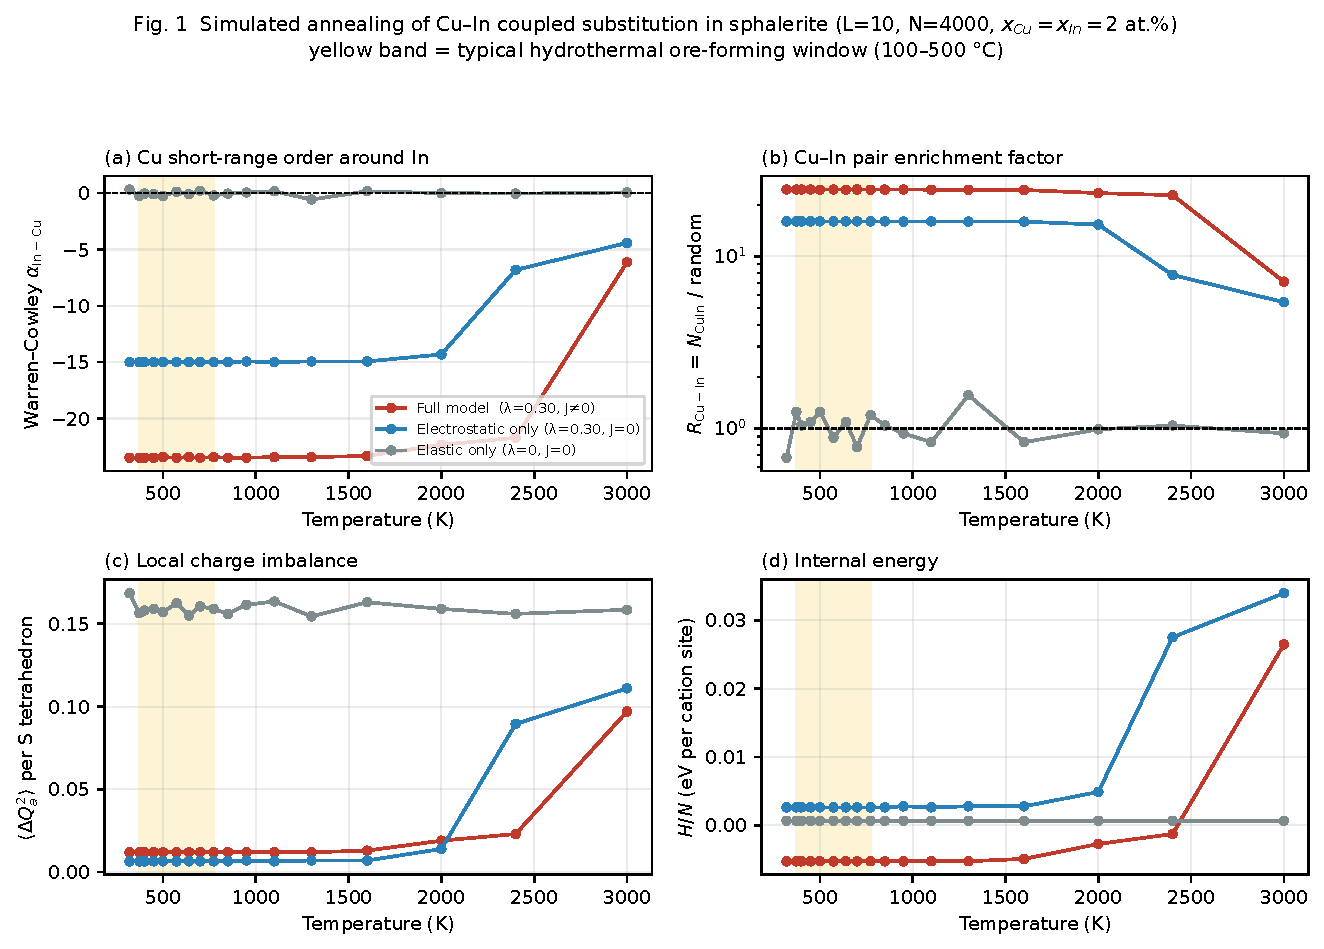
\includegraphics[width=\textwidth]{fig1_annealing.pdf}
\caption{Simulated annealing of Cu--In coupled substitution ($L = 10$,
$N = 4000$, $x_{\mathrm{Cu}} = x_{\mathrm{In}} = 2$~at.\%). Red, full model
($\lambda = 0.30$~eV, $J \neq 0$); blue, electrostatic only
($\lambda = 0.30$~eV, $J = 0$); grey, elastic only ($\lambda = 0$, $J = 0$).
Shaded band, hydrothermal ore-forming window (100--500$\,^\circ$C).
(a)~Warren--Cowley short-range order parameter $\aInCu$; dashed line marks the
random-solution value. (b)~Cu--In pair enrichment factor $\RCuIn$, logarithmic
scale. (c)~Mean squared tetrahedral charge deviation $\langle \dQ_a^2 \rangle$;
the elastic-only curve coincides with the analytic random value $8x = 0.160$.
(d)~Internal energy per cation site.}
\label{fig:anneal}
\end{figure}

\subsection{The ordering crossover lies far above the ore-forming window}
\label{sec:crossover}

The temperature dependence in Fig.~\ref{fig:anneal}a,b is that of a sharp but
continuous crossover rather than a gradual drift. In Experiment A3 the
enrichment factor rises from 5.4 at 3000~K ($\Theta = 0.86$) through 7.8 at
2400~K ($\Theta = 0.69$) to 15.3 at 2000~K ($\Theta = 0.57$), and is within 5\%
of its saturated value by 1600~K ($\Theta = 0.46$). Experiment A1, whose
additional chemical term deepens the effective pair binding, crosses over some
400--600~K higher. Locating the crossover at $\Theta^* \approx 0.6$--0.8, i.e.\
at $k_BT^* \approx 0.3$--0.4 times the pair binding energy $2\lambda$, is
consistent with the mean-field expectation for a system whose ordering is
controlled by a single nearest-neighbour bond energy.

The geological consequence is direct and, we suggest, the single most important
result of this paper: the entire hydrothermal ore-forming window
($\Theta = 0.11$--0.22, shaded band in Fig.~\ref{fig:anneal}) lies a factor of
three to seven \emph{below} the crossover. Over the whole of that window the
order parameters are flat to within the resolution of the calculation ($\aInCu$
varies by 0.05 between 773~K and 373~K in Experiment A1; see the caveat below).
Cu--In short-range
order in sphalerite is therefore not a low-temperature refinement that switches
on at some threshold within the ore system; it is saturated everywhere that
sphalerite forms, and its magnitude carries essentially no temperature
information.

\emph{Caveat added in version 2.} The flatness quoted above is measured on the
annealing protocol, which Section~\ref{sec:ergodicity} shows to be
under-converged by about 2\% at 573~K. A preliminary replica-exchange scan
across 373--773~K returns $\aInCu = -23.8 \pm 0.5$, consistent with flatness and
with the corrected 573~K value, but that scan achieved too few replica round
trips to be quoted as a converged result. The qualitative conclusion --- that the
crossover lies far above the ore-forming window, so short-range order is
saturated throughout it --- rests on the position of the crossover at
$\Theta^* \approx 0.6$--0.8, which is measured where the acceptance ratio is high
and equilibration is not in question. A fully converged re-measurement of the
window is deferred to future work.

\subsection{Robustness to the value of \texorpdfstring{$\lambda$}{lambda}}
\label{sec:lambdascan}

Experiment B scans $\lambda$ at fixed $T = 573$~K with $J = 0$, three
independent seeds per value (Fig.~\ref{fig:lambda}). The enrichment factor rises
steeply from $R = 1.06 \pm 0.20$ at $\lambda = 0$ through $R = 3.94 \pm 0.20$ at
0.05~eV to $R = 15.68 \pm 0.07$ at 0.10~eV, and is thereafter saturated: all
values in $0.10 \le \lambda \le 0.50$~eV lie between $R = 15.7$ and $R = 21.1$,
with seed-to-seed dispersion ($\pm 3.2$ to $\pm 3.8$ for
$\lambda \ge 0.15$~eV) exceeding any systematic trend.

Two conclusions follow. First, the dielectric estimate of Eq.~\eqref{eq:lambda},
$\lambda \in [0.227, 0.368]$~eV (green band in Fig.~\ref{fig:lambda}), lies
wholly within the saturated regime, so the principal result is insensitive to
the choice between the static and high-frequency dielectric constants. It is
also insensitive to the neglect of explicit Debye screening: even reducing
$\lambda$ by a factor $e^{-1}$ to 0.083~eV --- the most pessimistic correction
consistent with $\ell_D \simeq d_{NN}$ --- leaves $R$ above 10, and a full order
of magnitude of enrichment survives down to $\lambda \approx 0.07$~eV. The
qualitative conclusion is therefore stable across roughly a sevenfold range in
the only inferred parameter of the model.

Second, and less favourably, the saturation means that the present simulations
cannot resolve a threshold in $\lambda$, and the large seed-to-seed dispersion
above 0.15~eV reflects nucleation stochasticity rather than physics. Both are
consequences of the finite box, discussed in Section~\ref{sec:boundary}.

\begin{figure}[htbp]
\centering
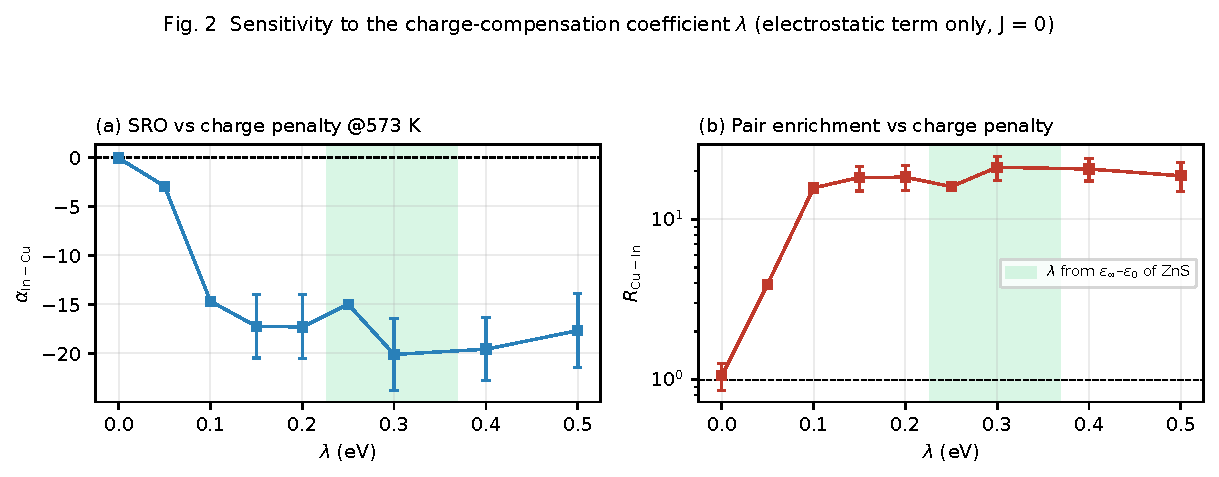
\includegraphics[width=0.92\textwidth]{fig2_lambda_scan.pdf}
\caption{Sensitivity to the charge-compensation coefficient $\lambda$ at 573~K
with $J = 0$; symbols are means of three independent seeds, error bars their
standard deviation. Green band, the interval $\lambda \in [0.227, 0.368]$~eV
predicted by Eq.~\eqref{eq:lambda} from the static and high-frequency dielectric
constants of ZnS. (a)~$\aInCu$. (b)~$\RCuIn$, logarithmic scale.}
\label{fig:lambda}
\end{figure}

\subsection{Bond-resolved statistics carry a heterovalent signature}
\label{sec:bonds}

The full bond census of the Experiment A1 configuration at 373~K
(Table~\ref{tab:bonds}) resolves the ordering into its components.
Solute--solute bonds of every kind are strongly enriched --- the solute
sublattice as a whole is aggregated by a factor of 16.8 --- but the enrichment is
markedly anisotropic with respect to valence. Heterovalent Cu--In bonds are
enriched 24.5-fold, whereas homovalent Cu--Cu and In--In bonds are enriched only
9.0- and 9.2-fold. The ratio of heterovalent to homovalent enrichment, 2.70, is
the direct fingerprint of $E_c$: a Cu--In bond carries
$\delta q_i \delta q_j = -1$ and is stabilised by $2\lambda$, whereas a Cu--Cu or
In--In bond carries $\delta q_i \delta q_j = +1$ and is destabilised by the same
amount, so homovalent contacts occur only as a by-product of aggregation rather
than as a driving force.

On average each In atom is surrounded by 5.88 Cu atoms out of its twelve cation
neighbours, against a random expectation of 0.24.

\begin{table}[htbp]
\centering
\caption{First-neighbour bond census, Experiment A1 at 373~K (24\,000 bonds
total).}
\label{tab:bonds}
\small
\begin{tabular}{lrrr}
\toprule
Bond type & Observed & Random expectation & Enrichment \\
\midrule
Cu--In & 470 & 19.2 & 24.5 \\
Cu--Cu & 86 & 9.6 & 9.0 \\
In--In & 88 & 9.6 & 9.2 \\
Zn--Cu & 318 & 921.6 & 0.35 \\
Zn--In & 314 & 921.6 & 0.34 \\
Zn--Zn & 22\,724 & 22\,118 & 1.03 \\
\midrule
all solute--solute & 644 & 38.4 & 16.8 \\
\bottomrule
\end{tabular}
\end{table}

\subsection{Condensation into a single solute nanodomain}
\label{sec:clusters}

Union--find analysis of the 373~K configurations (Fig.~\ref{fig:cluster}a,
Table~\ref{tab:clusters}) shows that the short-range order is accompanied by
complete spatial condensation. In the elastic-only control the 160 solute atoms
are dispersed across 120 clusters of mean size 1.33, of which 81\% are isolated
monomers --- the expected percolation statistics of a random 4~at.\% solute
population on an fcc lattice. In both Experiments A1 and A3 the same 160 atoms
form a \emph{single} connected cluster. The corresponding slab projections
(Fig.~\ref{fig:cluster}b,c) display the contrast directly.

\begin{table}[htbp]
\centering
\caption{Solute cluster statistics at 373~K.}
\label{tab:clusters}
\small
\begin{tabular}{lrrrr}
\toprule
Experiment & clusters & largest & mean size & monomer fraction \\
\midrule
A1 full & 1 & 160 & 160.0 & 0.00 \\
A3 electrostatic only & 1 & 160 & 160.0 & 0.00 \\
A2 elastic only & 120 & 5 & 1.33 & 0.81 \\
\bottomrule
\end{tabular}
\end{table}

The internal structure of this domain deserves attention, because it is not the
ideal roquesite ordering predicted analytically in
Section~\ref{sec:groundstate}. Resolving the first coordination shell of In in
Experiment A1 gives 0.490 Cu, 0.183 In and 0.327 Zn, against 0.667 Cu, 0.333 In
and 0 Zn for bulk chalcopyrite-type ordering. Two distinct discrepancies are
present. The Zn fraction of 0.327 reflects the large surface-to-volume ratio of
a 160-atom domain and would fall towards zero for larger clusters. The Cu:In
ratio within the solute shell, 2.68 against the ideal 2.00, is a genuine
departure from the ordered ground state, and is consistent with the residual
$\langle \dQ_a^2\rangle = 0.012 > 0$. We therefore describe the simulated object
as a \emph{charge-compensated roquesite precursor} rather than as roquesite: the
model reproduces the condensation and the heterovalent bonding rule, but at this
box size it does not reach the fully ordered $E_c = 0$ state.

\emph{Added in version 2.} The two Hamiltonians produce structurally distinct
domains, not merely different degrees of the same ordering. Under
electrostatics alone the In first shell contains 0.320 Cu, no In at all, and
0.680 Zn: an open, strictly alternating network in which no two solutes of like
charge are neighbours. The full model gives a denser domain, 0.500 Cu / 0.188 In
/ 0.312 Zn. Neither is bulk chalcopyrite ordering, which would give 0.667 / 0.333
/ 0; both are surface-dominated at 160 atoms. The origin of the difference is
analysed in Section~\ref{sec:jdiagnostic}.

\begin{figure}[htbp]
\centering
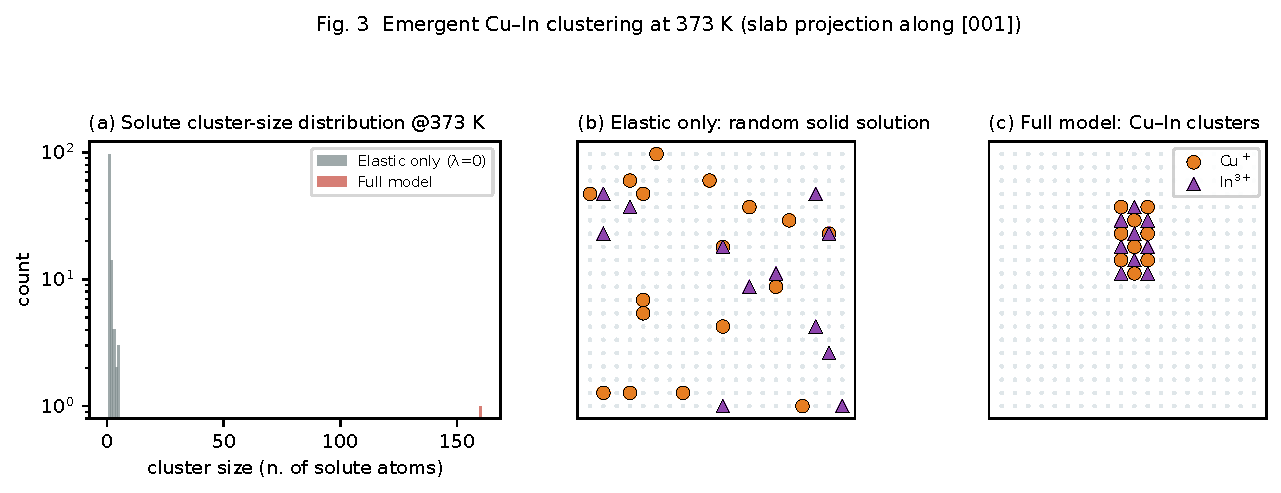
\includegraphics[width=\textwidth]{fig3_cluster.pdf}
\caption{Solute aggregation at 373~K. (a)~Cluster-size distribution from
union--find analysis of first-neighbour connectivity; grey, elastic-only control
(120 clusters, 81\% monomers); red, full model (a single 160-atom cluster).
(b,\,c)~Projections of a two-cell slab along $[001]$ for the elastic-only
control and the full model respectively; small grey symbols, Zn; orange circles,
Cu; purple triangles, In.}
\label{fig:cluster}
\end{figure}

\subsection{Equilibrium versus kinetic arrest}
\label{sec:ergodicity}

Because the acceptance ratio falls to $\sim 10^{-5}$ below 1300~K, the plateau
of Section~\ref{sec:crossover} could in principle be an artefact of
configurational freezing rather than a thermodynamic saturation. Experiment D
addresses this (Fig.~\ref{fig:ergo}). A trajectory quenched from a random
configuration straight to 573~K and a trajectory pre-annealed through 2000,
1400, 1000 and 800~K converge to $\aInCu = -23.17$ and $-23.48$ respectively ---
a difference of 0.31, or 1.3\% of the value --- and both order parameters are
stationary over the final $1.2\times10^4$ sweeps.

A residual difference does remain in the energy: the quenched trajectory settles
at $-0.00211$~eV per site against $-0.00528$~eV for the pre-annealed one
(Fig.~\ref{fig:ergo}b). The two configurations are thus equivalent at the level
of pair statistics but not at the level of total energy, the quenched state
lying 3.2~meV per site --- 12.7~eV over the box, or 79~meV per solute atom ---
above the annealed one.

\subsubsection*{Correction (version 2): the two-trajectory test was not
sufficient}

Version 1 of this paper concluded from the agreement of these two trajectories
that the low-temperature plateau was thermodynamic in origin. That inference was
not warranted, and subsequent work with a stronger sampler shows why.

Replica-exchange (parallel-tempering) sampling was applied to the same
Hamiltonian, box and composition, with an adaptively constructed ladder of
replicas spanning 573~K to 2200--3000~K and configurations exchanged between
adjacent replicas. From a quenched start, and within the same total sweep budget
that leaves plain Kawasaki dynamics at $-0.00271$~eV per site, replica exchange
reaches $-0.00605$~eV per site: \textbf{0.77~meV per site --- 3.1~eV over the
box --- below the pre-annealed state}, which was the lowest state version 1
attained. The result is reproduced by independent runs with different seeds,
different ladder lengths and different exchange frequencies, five configurations
of which agree on the energy to 0.055~meV per site.

Both trajectories of Experiment D were therefore metastable. Two independent
trajectories agreeing with one another is evidence of nothing when both are
trapped in the same basin, and version 1 drew a stronger conclusion from that
agreement than the data could support. The metastability that version 1 did
report, 3.2~meV per site between the quenched and annealed states, was real but
was itself an underestimate of the distance to equilibrium.

The corrected values at 573~K appear in Table~\ref{tab:573}. Relative to
version~1 they shift $\aInCu$ from $-23.48$ to $-24.00$, $\RCuIn$ from 24.48 to
25.00, and the fraction of local charge imbalance removed from 92.4\% to
93.7\%: a systematic 2\% under-convergence, in the direction of insufficient
ordering, as expected. Solute condensation into a single 160-atom cluster is
unchanged.

Two further points bear on the rest of the paper. First, the solute-shell
composition Cu:In moves only from 2.68 to 2.67 against the ideal 2.00, so the
departure from roquesite ordering identified in Section~\ref{sec:clusters} is
\emph{not} a sampling artefact, and the diagnostic built on it in
Section~\ref{sec:jdiagnostic} stands. Second, the elastic-only control
(Experiment A2) has an acceptance ratio of 0.978 and equilibrates freely, so it
requires no correction; the conclusion of Section~\ref{sec:elastic} is
unaffected.

\paragraph{The electrostatic-only calculation needs no correction.}
Experiment A3 might have been expected to suffer a comparable 2\%
under-convergence. It does not. Replica exchange applied to A3, with a ladder
built for that Hamiltonian and a production run achieving \textbf{13 replica
round trips}, returns $\aInCu = -14.99 \pm 0.00$, $\RCuIn = 15.99$,
$\langle \dQ_a^2\rangle = 0.0065 \pm 0.0000$ and $H/N = +0.00262$~eV per site:
the published annealing values, to every digit reported. Three further ladders
with tops at 2000, 2400 and 2800~K and lengths of 20, 26 and 28 replicas agree
on the energy to 0.001~meV per site. The sixteenfold enrichment and the 96\%
removal of local charge imbalance quoted in the abstract therefore stand as
measured, not as an order-of-magnitude estimate.

The same protocol applied to A1 gives $\aInCu = -23.96 \pm 0.01$ and
$H/N = -0.00604$~eV per site, confirming the version~2 correction, but achieves
only 5 round trips against A3's 13 in the same computational budget.

\paragraph{Where the metastability comes from.} The two Hamiltonians differ only
in $J_{\alpha\beta}$, so the contrast localises the difficulty precisely: the
sampling problem that version~1 ran into is caused by the hypothetical covalent
term, not by the charge-compensation term. On the pure $E_c$ landscape the
system anneals to equilibrium without difficulty. The mechanism is set out in
Section~\ref{sec:jdiagnostic}.

The methodological lesson is worth stating plainly, because the error is easy to
repeat: in a system with an acceptance ratio of $10^{-5}$, the convergence of two
trajectories towards each other is not a test of equilibration. What is needed is
a sampler capable of crossing the barriers, and a diagnostic --- such as the
replica round-trip count --- that measures whether it is actually doing so.

\begin{figure}[htbp]
\centering
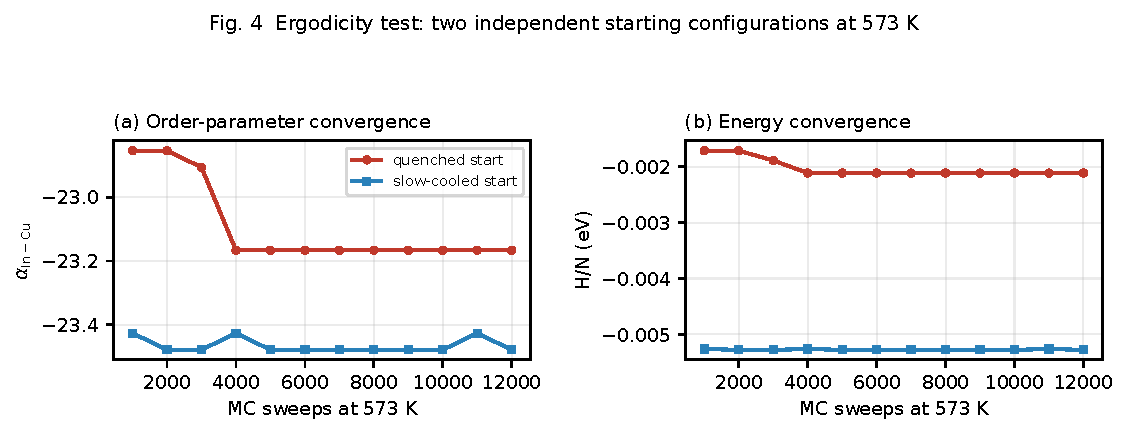
\includegraphics[width=0.86\textwidth]{fig4_ergodicity.pdf}
\caption{Test of equilibration at 573~K (Experiment D). Red circles, trajectory
quenched directly from a random configuration; blue squares, trajectory
pre-annealed through 2000, 1400, 1000 and 800~K. (a)~Convergence of $\aInCu$;
the two trajectories agree to 1.3\%. (b)~Convergence of the internal energy; the
quenched state remains 3.2~meV per site above the annealed one, the model's
signature of configurational metastability.}
\label{fig:ergo}
\end{figure}

%==============================================================================
\section{Discussion}

\subsection{The Cu--In correlation as a thermodynamic necessity}

The near-unity Cu:In molar ratio recorded by LA-ICP-MS in In-bearing sphalerite
from a wide range of deposit types is conventionally read as evidence for the
coupled substitution of Eq.~\eqref{eq:coupled}, with the coupling itself treated
as an empirical observation to be recorded rather than a quantity to be derived.
The results above allow a stronger statement. Starting from the zinc-blende
topology, formal ionic charges, and the measured dielectric constant of ZnS ---
with no fitted parameter and no input describing Cu--In affinity --- the model
yields a pair binding energy of $-2\lambda \approx -0.45$ to $-0.73$~eV
(Eq.~\eqref{eq:binding}), a sixteenfold enrichment of Cu--In nearest-neighbour
bonds at $300\,^\circ$C, and a ground state that is exactly the roquesite cation
ordering. The 1:1 correlation is not a contingent feature of ore-fluid
chemistry; it is what local electroneutrality on this particular lattice
topology requires.

Three subsidiary observations sharpen the claim. First, the effect is
specifically electrostatic: the elastic terms, retained at full strength in
Experiment A2, produce no measurable ordering whatever, confirming Hypothesis H1
within the model and predicting that Ag--In coupling, with its twentyfold larger
misfit, should behave qualitatively differently. Second, the effect is
valence-resolved: heterovalent bonds are enriched 2.7 times more strongly than
homovalent ones, which is the signature of $\delta q_i \delta q_j$ and not of
generic solute clustering. Third, the effect is saturated across the entire
temperature range in which sphalerite forms, so no ore-forming environment is
expected to host In as a genuinely random dilute solid solution.

\subsection{A diagnostic for the covalent term}
\label{sec:jdiagnostic}

The comparison between Experiments A1 and A3 yields an unanticipated and
potentially useful result. Adding $J_{\mathrm{Cu\text{-}In}} = -0.10$~eV raises
the apparent Cu--In enrichment from 16.0 to 24.5 --- but it simultaneously
\emph{degrades} local electroneutrality, with $\langle \dQ_a^2 \rangle$ rising
from 0.0065 to 0.0120 (Table~\ref{tab:573}). \emph{The mechanism given in version 1 of this paper was wrong, and the
converged Experiment A3 reported above shows why.} It was there argued that
perfect charge compensation requires four homovalent neighbours out of twelve,
and that $J_{\mathrm{Cu\text{-}Cu}} = J_{\mathrm{In\text{-}In}} = +0.05$~eV
penalises exactly those contacts, driving the In shell away from the ideal
Cu:In~$=2.00$. But A3, which contains no $J$ at all, departs from that ideal
\emph{further}, not less: its In first shell contains 0.320 Cu and
\textbf{zero} In.

The bond census resolves it. Writing $E_c$ in the pair form of
Eq.~\eqref{eq:Ecpair}, at fixed composition the configurational part is
$2\lambda \sum_{\langle ij\rangle} \delta q_i \delta q_j$, so $E_c$ is minimised
by maximising the excess of heterovalent over homovalent solute contacts.
Experiment A3 does exactly that: 307 Cu--In bonds and no homovalent solute
contacts whatever, giving $\sum \delta q_i \delta q_j = -307$ and
$E_c = 7.80$~eV. Experiment A1 instead has 480 Cu--In bonds together with about
90 Cu--Cu and 90 In--In, giving $-300$ and $E_c = 12.00$~eV. Both reconstructions
reproduce $\lambda N \langle \dQ_a^2\rangle$ exactly.

So $J_{\mathrm{Cu\text{-}In}} = -0.10$~eV buys a 56\% denser Cu--In network at
the cost of 4.2~eV of electrostatic energy, and the homovalent contacts are not
something $J$ tolerates but something the denser packing \emph{forces}: the fcc
cation sublattice contains 24 triangles through every site, so a compact solute
domain cannot be two-coloured without homovalent edges. The competition between
$E_c$, which favours an open alternating network, and $J$, which favours dense
aggregation, is also what makes the A1 landscape rugged and the A3 landscape
smooth, and hence what caused the equilibration failure of version~1.

The discriminant itself survives this correction, and is now measured at
converged sampling rather than inferred. The two quantities $\RCuIn$ and
$\langle \dQ_a^2 \rangle$ respond to $E_c$ in the same direction but to $J$ in
opposite directions: switching $J$ on takes $\RCuIn$ from 15.99 to 25.00 while
taking $\langle \dQ_a^2\rangle$ from 0.0065 to 0.0100. A third, independent
signature has now been added --- the ruggedness of the energy landscape, visible
as a factor of 2.6 fewer replica round trips at equal computational cost. Measurements sensitive to
short-range order and to local charge state --- EXAFS coordination numbers,
XANES edge positions, or the bond-valence sums extractable from high-resolution
structural refinement --- could therefore constrain the sign and magnitude of the
non-electrostatic term without a full \textit{ab initio} calculation.

\subsection{Implications for exploration and resource evaluation}
\label{sec:exploration}

We set out four implications, in decreasing order of confidence. All are
predictions of a model calibrated at a single composition on a small box, and
require empirical validation.

\paragraph{(i) Cu availability, not In availability, should limit In tenor.}
If In incorporation must be locally charge-balanced, and if the Cu-compensated
route is favoured over the vacancy route by $8\lambda \approx 2.4$~eV
(Section~\ref{sec:competition}), then the achievable In content of sphalerite is
capped by the supply of a monovalent compensator. The practical corollary is
that In prospectivity should be assessed against the \emph{coupled} availability
of Cu and In in the mineralising system rather than against In anomalies alone
--- favouring, for example, settings in which Cu-rich and Zn-rich assemblages are
spatially and temporally linked. This reframes an empirical association already
noted in deposit-type meta-analyses as a consequence of lattice thermodynamics.

\paragraph{(ii) Vacancy compensation should be diagnostic of Cu-poor systems.}
Equation~\eqref{eq:crossover} makes the competition quantitative. In-rich but
Cu-poor sphalerite should therefore be measurably cation-deficient, and should
depart from the 1:1 Cu:In line in a specific direction. This is testable with
existing EPMA and LA-ICP-MS data provided that stoichiometry is reported, and
constitutes the sharpest near-term falsification test of the model.

\paragraph{(iii) Trace-element short-range order is not a geothermometer.}
Because the order parameters are flat across the entire ore-forming window
(Section~\ref{sec:crossover}), the degree of Cu--In association recorded by a
natural sphalerite carries almost no information about its formation
temperature. More seriously, the configuration retains a memory of its \emph{cooling path}:
quenched and slowly cooled states differ by 79~meV per solute atom while being
indistinguishable in pair statistics, and replica exchange shows that even the
slowly cooled state lies a further 19~meV per solute atom above equilibrium
(Section~\ref{sec:ergodicity}). The metastability is therefore deeper than
version~1 reported, which strengthens rather than weakens this point. Any attempt to read formation conditions from
trace-element site occupancy must therefore contend with a configurational
closure temperature distinct from the growth temperature, and pair statistics
alone will not resolve it.

\paragraph{(iv) Spatial heterogeneity should be intrinsic, not sampling noise.}
The condensation of all solutes into a single domain
(Section~\ref{sec:clusters}) is a nucleation-controlled process, and the large
seed-to-seed dispersion of Experiment B is its statistical expression. If this
behaviour survives at realistic length scales --- which the present box cannot
establish --- then In should be distributed heterogeneously within individual
sphalerite grains, and bulk assay values would average over a distribution
rather than measure a representative concentration. The practical implication is
that micro-analytical mapping is not merely a refinement of bulk assay for In
resources but measures a different quantity. We flag this as the most
speculative of the four.

A further consequence concerns the thermodynamic formalism itself. Partition
coefficients for In between sphalerite and hydrothermal fluid are ordinarily
modelled assuming ideal dilute mixing, i.e.\ full configurational entropy
$-k_B \sum x_\alpha \ln x_\alpha$. The enrichment factors reported here imply
that this entropy is substantially overestimated at ore-forming temperatures,
and hence that the In solubility inferred from such models is too high. The
canonical simulations presented here cannot quantify the correction, because
composition is held fixed by construction; doing so requires a grand-canonical
treatment.

\subsection{Toward the solid-solution versus nanoinclusion boundary}
\label{sec:boundary}

The long-standing question of whether In in sphalerite resides in true solid
solution or in nanoscale inclusions is precisely the question that the present
calculations \emph{cannot} answer, and it is worth being explicit about why.

At $N = 4000$ and 4~at.\% total solute, the 160 solute atoms are sufficient to
form exactly one domain of the size that the model wants to build. The system
therefore has no way to express an intermediate state: once nucleation occurs,
the entire solute budget is consumed, the order parameters saturate, and the
distinction between ``dispersed pairs'', ``several competing nuclei'' and ``a
single inclusion'' is lost. This is the origin of the saturation of
Fig.~\ref{fig:lambda} above $\lambda = 0.10$~eV and of the seed-to-seed
dispersion above 0.15~eV; both are finite-size artefacts and neither should be
interpreted physically.

Four requirements follow for any study aiming to settle the question.
(a)~\emph{Box size.} Resolving a genuine dilute limit alongside competing nuclei
requires of order $50^3$ cells ($5\times10^5$ sites), which raises the solute
population by two orders of magnitude and permits a meaningful cluster-size
distribution. (b)~\emph{Sampling.} The acceptance collapse to $10^{-5}$ makes
simple Kawasaki dynamics inadequate at ore-forming temperatures; parallel
tempering or cluster moves generalising the Wolff construction to the
four-state charged model will be required, and $10^8$--$10^{10}$ trial moves
will be needed per state point. (c)~\emph{Composition.} A scan across
$x_{\mathrm{In}}$ from $10^{-3}$ to $5\times10^{-2}$ is needed to locate the
solvus, which is the quantity of economic interest.
(d)~\emph{Parameterisation.} $J_{\alpha\beta}$, $E^f_V$ and the Fe-dependence of
$\epsilon_r$ must come from first-principles calculation, since
Section~\ref{sec:jdiagnostic} shows that $J$ controls not only the magnitude of
the enrichment but the internal ordering of the resulting domain.

The present paper contributes to that programme in three ways: it supplies the
Hamiltonian and its exact analytic limits, it establishes that the electrostatic
term alone suffices to drive the transition, and it identifies precisely which
observables are and are not resolvable at small box size.

\subsection{Limitations}

Beyond the finite-size issues above, four limitations should be borne in mind
when comparing with natural samples.

First, Fe is absent from the model, whereas natural sphalerite commonly contains
up to 10~mol\% FeS. Fe$^{2+}$ is isovalent with Zn$^{2+}$ and so does not enter
$E_c$ directly, but Fe~$3d$ states modify both the dielectric response that
fixes $\lambda$ through Eq.~\eqref{eq:lambda} and the substitution energies of
Eq.~\eqref{eq:dft}. The sign of the effect is not obvious \textit{a priori}.

Second, the treatment is a rigid-lattice one. Atomic relaxation is represented
only through the continuum expressions of Eqs.~\eqref{eq:eshelby} and
\eqref{eq:dipole}, which are in any case of marginal validity for large misfits;
the Eshelby form should not be applied to Ag$^+$ ($\varepsilon = 0.67$) without
independent verification, despite the comparison drawn above.

Third, Monte Carlo sweeps are not physical time. The freezing documented in
Section~\ref{sec:ergodicity} is a property of the sampling algorithm, and
although we have argued that it has a natural geological analogue in
configurational closure, the model as formulated makes no kinetic predictions
and cannot be used to estimate diffusion-limited closure temperatures.

Fourth, sampling below about 1300~K is difficult, and version~1 of this paper
underestimated how difficult. The annealing results reported here are
under-converged by roughly 2\% in the order parameters; the corrected 573~K
values obtained by replica exchange are given in Table~\ref{tab:573}, while the
remaining tables and figures retain the annealing values so that the internal
comparison between Experiments A1, A2 and A3 stays on a common footing. Any
extension of this work to larger boxes or lower temperatures should use replica
exchange from the outset and report replica round-trip counts as the convergence
diagnostic.

Fifth, all calculations are at a single composition,
$x_{\mathrm{Cu}} = x_{\mathrm{In}} = 2$~at.\%, which lies at the upper end of
natural In contents. Behaviour in the ppm range --- where the great majority of
economically relevant sphalerite sits --- has not been sampled.

%==============================================================================
\section{Conclusions}

\begin{enumerate}\itemsep3pt
\item An exact topological property of the zinc-blende structure --- that two
      nearest-neighbour cations share precisely one bridging anion --- allows a
      local electroneutrality functional on the sulphur tetrahedra to be reduced
      without approximation to a nearest-neighbour pair interaction on the
      cation sublattice, Eq.~\eqref{eq:Ecpair}.

\item The coefficient of that interaction is fixed by the dielectric constant of
      ZnS rather than fitted, $\lambda \in [0.227, 0.368]$~eV, giving a Cu--In
      pair binding energy of $-2\lambda \approx -0.45$ to $-0.73$~eV.

\item The ground state of the charge-compensation term at Cu:In~$=1$:1 is
      exactly the roquesite ($\mathrm{CuInS_2}$) cation ordering, recovered
      without any structural input describing that phase. The ground state is
      degenerate across orderings satisfying the two-Cu-two-In tetrahedral rule,
      so polytype selection requires the chemical and elastic terms.

\item Monte Carlo simulation confirms these predictions. Electrostatics alone
      enriches Cu--In nearest-neighbour bonds sixteenfold at $300\,^\circ$C and
      removes 96\% of the local charge imbalance; heterovalent bonds are
      enriched 2.7 times more strongly than homovalent ones. Elastic terms,
      retained at full strength in a control, produce no detectable ordering.

\item The ordering crossover lies at $\Theta^* \approx 0.6$--0.8, a factor of
      three to seven above the entire hydrothermal window. Cu--In short-range
      order is therefore saturated wherever sphalerite forms and carries no
      thermometric information.

\item The Cu-compensated route is favoured over vacancy compensation by
      $8\lambda \approx 2.4$~eV, giving the falsifiable criterion of
      Eq.~\eqref{eq:crossover}: vacancy compensation should be confined to
      Cu-poor systems and detectable as cation deficiency.

\item Finite box size prevents resolution of the solid-solution versus
      nanoinclusion boundary. Settling that question requires $50^3$-cell boxes,
      enhanced sampling, a composition scan, and first-principles
      parameterisation of the chemical term.
\end{enumerate}

%==============================================================================
\section*{Data and code availability}

The complete source code, the numerical results underlying all figures and
tables, and the scripts that regenerate every figure from scratch are openly
available at
\url{https://github.com/Ruqing1963/sphalerite-lattice-mc}. The repository
includes the verification and validation suite of Section~\ref{sec:vv}, which
reproduces every analytic limit quoted in this paper. Code is released under the
MIT licence and data under CC~BY~4.0. The replica-exchange sampler used for the
version~2 correction, together with the ladder-calibration and benchmarking
scripts, is part of the same repository.

\section*{Author contributions}

\textbf{He Yu:} conceptualisation, geological framing, validation, writing ---
review and editing. \textbf{Ruqing Chen:} methodology, formal analysis,
software, investigation, visualisation, writing --- original draft.
\textbf{Huanzhang Lu:} critical review of the full manuscript, key
revision suggestions, and participation in multiple rounds of revision.

\section*{Declaration of competing interests}

The authors declare no competing financial or personal interests.

\section*{Funding}

This study was funded by the Hezhou Municipal Scientific Research and
Development Program (Project Nos.\ 2024143, 2024141 and 2024104).

%==============================================================================
\begin{thebibliography}{99}
\itemsep2pt

\bibitem[Belissont et al.(2014)]{belissont2014}
Belissont, R., Boiron, M.-C., Luais, B., Cathelineau, M. (2014) LA-ICP-MS
analyses of minor and trace elements and bulk Ge isotopes in zoned Ge-rich
sphalerites from the Noailhac--Saint-Salvy deposit (France). \textit{Geochimica
et Cosmochimica Acta} 126, 518--540.

\bibitem[Berlincourt et al.(1963)]{berlincourt1963}
Berlincourt, D., Jaffe, H., Shiozawa, L.R. (1963) Electroelastic properties of
the sulfides, selenides, and tellurides of zinc and cadmium. \textit{Physical
Review} 129, 1009--1017.

\bibitem[Cook et al.(2009)]{cook2009}
Cook, N.J., Ciobanu, C.L., Pring, A., Skinner, W., Shimizu, M., Danyushevsky,
L., Saini-Eidukat, B., Melcher, F. (2009) Trace and minor elements in
sphalerite: A LA-ICPMS study. \textit{Geochimica et Cosmochimica Acta} 73,
4761--4791.

\bibitem[Cowley(1950)]{cowley1950}
Cowley, J.M. (1950) An approximate theory of order in alloys. \textit{Physical
Review} 77, 669--675.

\bibitem[Eshelby(1957)]{eshelby1957}
Eshelby, J.D. (1957) The determination of the elastic field of an ellipsoidal
inclusion, and related problems. \textit{Proceedings of the Royal Society A}
241, 376--396.

\bibitem[Frenzel et al.(2016)]{frenzel2016}
Frenzel, M., Hirsch, T., Gutzmer, J. (2016) Gallium, germanium, indium and other
trace and minor elements in sphalerite as a function of deposit type --- a
meta-analysis. \textit{Ore Geology Reviews} 76, 52--78.

\bibitem[Freysoldt et al.(2014)]{freysoldt2014}
Freysoldt, C., Grabowski, B., Hickel, T., Neugebauer, J., Kresse, G., Janotti,
A., Van de Walle, C.G. (2014) First-principles calculations for point defects in
solids. \textit{Reviews of Modern Physics} 86, 253--305.

\bibitem[Hoang(2019)]{hoang2019}
Hoang, K. (2019) Defect energy levels and persistent luminescence in Cu-doped
ZnS. \textit{Physical Review Materials} 3, 034604.

\bibitem[Johan(1988)]{johan1988}
Johan, Z. (1988) Indium and germanium in the structure of sphalerite: an example
of coupled substitution with copper. \textit{Mineralogy and Petrology} 39,
211--229.

\bibitem[Kawasaki(1966)]{kawasaki1966}
Kawasaki, K. (1966) Diffusion constants near the critical point for
time-dependent Ising models. \textit{Physical Review} 145, 224--230.

\bibitem[Li(1984)]{li1984}
Li, H.H. (1984) Refractive index of ZnS, ZnSe, and ZnTe and its wavelength and
temperature derivatives. \textit{Journal of Physical and Chemical Reference
Data} 13, 103--150.

\bibitem[Metropolis et al.(1953)]{metropolis1953}
Metropolis, N., Rosenbluth, A.W., Rosenbluth, M.N., Teller, A.H., Teller, E.
(1953) Equation of state calculations by fast computing machines.
\textit{Journal of Chemical Physics} 21, 1087--1092.

\bibitem[Moura et al.(2007)]{moura2007}
Moura, M.A., Botelho, N.F., de Mendon\c{c}a, F.C. (2007) The indium-rich
sulfides and rare arsenates of the Sn-In-mineralized Mangabeira A-type granite,
central Brazil. \textit{The Canadian Mineralogist} 45, 485--496.

\bibitem[Pauling(1929)]{pauling1929}
Pauling, L. (1929) The principles determining the structure of complex ionic
crystals. \textit{Journal of the American Chemical Society} 51, 1010--1026.

\bibitem[Shannon(1976)]{shannon1976}
Shannon, R.D. (1976) Revised effective ionic radii and systematic studies of
interatomic distances in halides and chalcogenides. \textit{Acta
Crystallographica} A32, 751--767.

\bibitem[Trofimov et al.(2020)]{trofimov2020}
Trofimov, N.D., Filimonova, O.N., Nickolsky, M.S., Abramova, V.D., Evstigneeva,
P.V., Kvashnina, K.O., Trigub, A.L., Chareev, D.A., Tagirov, B.R. (2020) The
state of copper, silver and indium in sphalerite studied by X-ray spectroscopy
of synthetic crystals and natural minerals. \textit{Journal of Alloys and
Compounds} 847, 156557.

\bibitem[USGS(2024)]{usgs2024}
U.S. Geological Survey (2024) \textit{Mineral Commodity Summaries 2024:
Indium}. U.S. Geological Survey, Reston, Virginia.

\bibitem[Werner et al.(2015)]{werner2015}
Werner, T.T., Mudd, G.M., Jowitt, S.M. (2015) Indium: key issues in assessing
mineral resources and long-term supply from linchpin polymetallic deposits.
\textit{Applied Earth Science} 124, 213--226.

\end{thebibliography}

\end{document}
